\documentclass{beamer}
\usepackage{ctex, hyperref}
\usepackage[T1]{fontenc}

% other packages
\usepackage{latexsym,amsmath,xcolor,multicol,booktabs,calligra}
\usepackage{graphicx,pstricks,listings,stackengine}

\author{Allenpandas}
\title{基于***的***方法研究(这是标题的位置)}
\subtitle{研究生论文开题报告(这是副标题的位置)}
\institute{北京交通大学·计算机与信息技术学院}
\date{2022年12月30日}
\usepackage{bjtu}

% defs
\def\cmd#1{\texttt{\color{red}\footnotesize $\backslash$#1}}
\def\env#1{\texttt{\color{blue}\footnotesize #1}}
\definecolor{deepblue}{rgb}{0,0,0.5}
\definecolor{deepred}{rgb}{0.6,0,0}
\definecolor{deepgreen}{rgb}{0,0.5,0}
\definecolor{halfgray}{gray}{0.55}

\lstset{
    basicstyle=\ttfamily\small,
    keywordstyle=\bfseries\color{deepblue},
    emphstyle=\ttfamily\color{deepred},    % Custom highlighting style
    stringstyle=\color{deepgreen},
    numbers=left,
    numberstyle=\small\color{halfgray},
    rulesepcolor=\color{red!20!green!20!blue!20},
    frame=shadowbox,
}


\begin{document}

\kaishu
% 每页根据frame标签来分割
\begin{frame}
    \titlepage
    \begin{figure}[htpb]
        \begin{center}
            
\includegraphics[width=0.2\linewidth]{pic/bjtu_logo.jpeg}
        \end{center}
    \end{figure}
\end{frame}


% 目录页
\begin{frame}
%使用tableofcontents命令可以自动生成目录
    \tableofcontents[sectionstyle=show,subsectionstyle=show/shaded/hide,subsubsectionstyle=show/shaded/hide]
\end{frame}


% 第一章
\section{课题背景}
% 第一节
\subsection{为什么使用Latex?}
\begin{frame}{Latex的优点}
    \begin{itemize}
        \item GitHub项目地址位于 \url{https://github.com/Allenpandas/BJTU-Beamer-Theme},如果有bug或者feature request可以去里面提issue
        \item "课题背景"是"章",用section表示
        \item "为什么使用Latex?"是"节",用subsection表示
        \item "Latex的优点"是"节"下面的标题(本页PPT的标题),可有可无。
    \end{itemize}
\end{frame}

\begin{frame}{}
    \begin{itemize}
        \item 如果想去掉每页的标题(如本页所示),只需从代码中去掉{frame}后面括号的内容即可。
    \end{itemize}
\end{frame}



% 第二章
\section{研究现状}
%\subsection{Beamer主题分类}
\begin{frame}
    \begin{itemize}
        \item 第二章叫“研究现状”,第二章的第二节叫“Beamer主题分类”。
        \item 如果不想在目录中显示“节”的包体,只需去掉{\color{red}{sebsection\{Beamer主题分类\}}} 这行代码即可       
    \end{itemize}
\end{frame}


% 第三章
\section{研究内容}
\subsection{如何用latex绘制表格}

\begin{frame}{下面是个表格的模板}
    \begin{table}[h]
        \centering
        \caption{Word和Latex的对比}
        \begin{tabular}{c|c}
        	            Microsoft\textsuperscript{\textregistered}  Word & \LaTeX \\
            \hline
            文字处理工具 & 专业排版软件 \\
            容易上手,简单直观 & 容易上手 \\
            所见即所得 & 所见即所想,所想即所得 \\
            高级功能不易掌握 & 进阶难,但一般用不到 \\
            处理长文档需要丰富经验 & 和短文档处理基本无异 \\
            花费大量时间调格式 & 无需担心格式,专心作者内容 \\
            公式排版差强人意 & 尤其擅长公式排版 \\
            二进制格式,兼容性差 & 文本文件,易读、稳定 \\
            付费商业许可 & 自由免费使用 \\
        \end{tabular}
    \end{table}
\end{frame}

\subsection{如何用latex插入公式}
\begin{frame}{两种公式举例}

    \begin{exampleblock}{无编号公式\footnote{无编号公式equation标签后面要加一个*;(当前这句话使用了一个脚标,脚标用footnote标签)}} % 加 * 
        \begin{equation*}
            \sin \alpha + \sin \beta =2 \sin \frac{\alpha + \beta}{2}\cos \frac{\alpha - \beta}{2}
        \end{equation*}
    \end{exampleblock}
    
    \begin{exampleblock}{有编号公式} % 加 * 
        \begin{equation}
           \frac{\sin A}{a}=\frac{\sin B}{b}=\frac{\sin C}{c}=\frac{1}{2R}        \end{equation}
    \end{exampleblock}
\end{frame}


\begin{frame}
    \begin{exampleblock}{遇到多行公式,可以使用equation标签也可以使用multline标签}
        % Taken from Mathmode.tex
        \begin{equation*}
            A_{m\times n}= \begin{bmatrix} a_{11}& a_{12}& \cdots & a_{1n} \\ a_{21}& a_{22}& \cdots & a_{2n} \\ \vdots & \vdots & \ddots & \vdots \\ a_{m1}& a_{m2}& \cdots & a_{mn} \end{bmatrix} =\left [ a_{ij}\right ]
        \end{equation*}
    \end{exampleblock}
\end{frame}



\begin{frame}{图形与分栏}
	% 左侧	
    \begin{minipage}[c]{0.4\linewidth}
    	\begin{itemize}
    		\item 制作Slide时,图文并茂更能吸引人,因此需要在适当的位置插入图片。
    		\item 使用minipage标签,可以实现分栏。
    	\end{itemize}
    \end{minipage}
%	\hspace{1cm}
    % 右侧
    \begin{minipage}{0.5\linewidth}
        \medskip
        %\hspace{2cm}
        \begin{figure}[h]
            \centering
            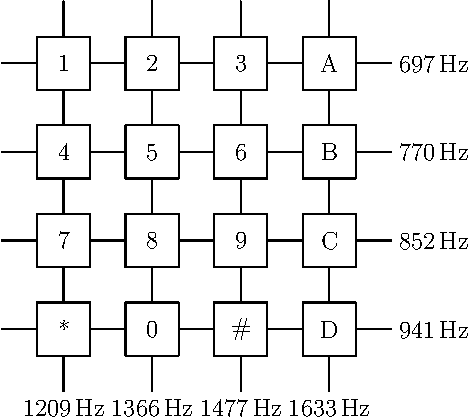
\includegraphics[height=.4\textheight]{pic/dtmf.pdf}
        \end{figure}
    \end{minipage}
\end{frame}












\begin{frame}[fragile]{\LaTeX{} 常用命令}
    \begin{exampleblock}{命令}
        \centering
        \footnotesize
        \begin{tabular}{llll}
            \cmd{chapter} & \cmd{section} & \cmd{subsection} & \cmd{paragraph} \\
            章 & 节 & 小节 & 带题头段落 \\\hline
            \cmd{centering} & \cmd{emph} & \cmd{verb} & \cmd{url} \\
            居中对齐 & 强调 & 原样输出 & 超链接 \\\hline
            \cmd{footnote} & \cmd{item} & \cmd{caption} & \cmd{includegraphics} \\
            脚注 & 列表条目 & 标题 & 插入图片 \\\hline
            \cmd{label} & \cmd{cite} & \cmd{ref} \\
            标号 & 引用参考文献 & 引用图表公式等\\\hline
        \end{tabular}
    \end{exampleblock}
    \begin{exampleblock}{环境}
        \centering
        \footnotesize
        \begin{tabular}{lll}
            \env{table} & \env{figure} & \env{equation}\\
            表格 & 图片 & 公式 \\\hline
            \env{itemize} & \env{enumerate} & \env{description}\\
            无编号列表 & 编号列表 & 描述 \\\hline
        \end{tabular}
    \end{exampleblock}
\end{frame}

\begin{frame}[fragile]{\LaTeX{} 环境命令举例}
    \begin{minipage}{0.5\linewidth}
\begin{lstlisting}[language=TeX]
\begin{itemize}
  \item A \item B
  \item C
  \begin{itemize}
    \item C-1
  \end{itemize}
\end{itemize}
\end{lstlisting}
    \end{minipage}\hspace{1cm}
    \begin{minipage}{0.3\linewidth}
        \begin{itemize}
            \item A
            \item B
            \item C
            \begin{itemize}
                \item C-1
            \end{itemize}
        \end{itemize}
    \end{minipage}
    \medskip
    \pause
    \begin{minipage}{0.5\linewidth}
\begin{lstlisting}[language=TeX]
\begin{enumerate}
  \item 巨佬 \item 大佬
  \item 萌新
  \begin{itemize}
    \item[n+e] 瑟瑟发抖
  \end{itemize}
\end{enumerate}
\end{lstlisting}
    \end{minipage}\hspace{1cm}
    \begin{minipage}{0.3\linewidth}
        \begin{enumerate}
            \item 巨佬
            \item 大佬
            \item 萌新
            \begin{itemize}
                \item[n+e] 瑟瑟发抖
            \end{itemize}
        \end{enumerate}
    \end{minipage}
\end{frame}

\begin{frame}[fragile]{\LaTeX{} 数学公式}
    \begin{columns}
        \begin{column}{.55\textwidth}
\begin{lstlisting}[language=TeX]
$V = \frac{4}{3}\pi r^3$

\[
  V = \frac{4}{3}\pi r^3
\]

\begin{equation}
  \label{eq:vsphere}
  V = \frac{4}{3}\pi r^3
\end{equation}
\end{lstlisting}
        \end{column}
        \begin{column}{.4\textwidth}
            $V = \frac{4}{3}\pi r^3$
            \[
                V = \frac{4}{3}\pi r^3
            \]
            \begin{equation}
                \label{eq:vsphere}
                V = \frac{4}{3}\pi r^3
            \end{equation}
        \end{column}
    \end{columns}
    \begin{itemize}
        \item 更多内容请看 \href{https://zh.wikipedia.org/wiki/Help:数学公式}{\color{purple}{这里}}
    \end{itemize}
\end{frame}

\begin{frame}[fragile]
    \begin{columns}
        \column{.6\textwidth}
\begin{lstlisting}[language=TeX]
    \begin{table}[htbp]
      \caption{编号与含义}
      \label{tab:number}
      \centering
      \begin{tabular}{cl}
        \toprule
        编号 & 含义 \\
        \midrule
        1 & 4.0 \\
        2 & 3.7 \\
        \bottomrule
      \end{tabular}
    \end{table}
    公式~(\ref{eq:vsphere}) 的
    编号与含义请参见
    表~\ref{tab:number}。
\end{lstlisting}
        \column{.4\textwidth}
        \begin{table}[htpb]
            \centering
            \caption{编号与含义}
            \label{tab:number}
            \begin{tabular}{cl}\toprule
                编号 & 含义 \\\midrule
                1 & 4.0\\
                2 & 3.7\\\bottomrule
            \end{tabular}
        \end{table}
        \normalsize 公式~(\ref{eq:vsphere})的编号与含义请参见表~\ref{tab:number}。
    \end{columns}
\end{frame}

\begin{frame}{作图}
    \begin{itemize}
        \item 矢量图 eps, ps, pdf
        \begin{itemize}
            \item METAPOST, pstricks, pgf $\ldots$
            \item Xfig, Dia, Visio, Inkscape $\ldots$
            \item Matlab / Excel 等保存为 pdf
        \end{itemize}
        \item 标量图 png, jpg, tiff $\ldots$
        \begin{itemize}
            \item 提高清晰度,避免发虚
            \item 应尽量避免使用
        \end{itemize}
    \end{itemize}
    \begin{figure}[htpb]
        \centering
        
\includegraphics[width=0.2\linewidth]{pic/bjtu_logo.jpeg}
        \caption{这个校徽就是矢量图}
    \end{figure}
\end{frame}


\section{计划进度}
\begin{frame}
    \begin{itemize}
        \item 一月:完成文献调研
        \item 二月:阅读论文:\cite{cao2019adversarial}(注意参考文献的写法)
        \item 三月:继续阅读论文:\cite{brunke2022safe}\cite{brunke2022safe}
    \end{itemize}
\end{frame}



\section{参考文献}

\begin{frame}[allowframebreaks]{参考文献列表}
    \bibliography{ref}
    \bibliographystyle{alpha}
    % 如果参考文献太多的话,可以像下面这样调整字体:
    % \tiny\bibliographystyle{alpha}
\end{frame}



% 致谢页
%\section{致谢}
\begin{frame}
    \begin{center}
        {\Huge\calligra 感谢各位的聆听}
    \end{center}
\end{frame}

\end{document}